\hypertarget{detector-model-kiukas-et-al.vs-pw}{%
\section{Detector model: Kiukas et al.~vs
PW}\label{detector-model-kiukas-et-al.vs-pw}}

\begin{lstlisting}[language=Python]
from sympy import *
# from sympy.physics.matrices import mdft
# from sympy.physics.quantum import TensorProduct
from sympy.physics.quantum.dagger import Dagger
from sympy.plotting import plot
import numpy as np
import matplotlib.pyplot as plt
\end{lstlisting}

\begin{lstlisting}[language=Python]
gamma = Symbol('gamma')
t = Symbol('t')
tprime = Symbol('t\'')
\end{lstlisting}

\begin{lstlisting}[language=Python]
def D(_gamma):
    return Rational(1, 2) * Matrix([
        [0, 0],
        [0, _gamma]
    ])
\end{lstlisting}

\begin{lstlisting}[language=Python]
H = Matrix ([
[0, 1] ,
[1, 0]
])
\end{lstlisting}

\begin{lstlisting}[language=Python]
init_printing ()
\end{lstlisting}

\begin{lstlisting}[language=Python]
H
\end{lstlisting}

\[\left[\begin{matrix}0 & 1\\1 & 0\end{matrix}\right]\]

\begin{lstlisting}[language=Python]
H.eigenvects()
\end{lstlisting}

\[\left [ \left ( -1, \quad 1, \quad \left [ \left[\begin{matrix}-1\\1\end{matrix}\right]\right ]\right ), \quad \left ( 1, \quad 1, \quad \left [ \left[\begin{matrix}1\\1\end{matrix}\right]\right ]\right )\right ]\]

It's manually seen that \(\langle H \rangle = 0\) and
\(\langle H^2 \rangle = 1\), therefore \(\sigma_{H} = 1\).

\begin{lstlisting}[language=Python]
def K(_gamma):
    return H - I*D(_gamma)
\end{lstlisting}

\begin{lstlisting}[language=Python]
K(gamma)
\end{lstlisting}

\[\left[\begin{matrix}0 & 1\\1 & - \frac{i \gamma}{2}\end{matrix}\right]\]

\begin{lstlisting}[language=Python]
def B(_gamma):
    return lambda t: exp(-I*K(_gamma)*t)
\end{lstlisting}

\begin{lstlisting}[language=Python]
def lossy_norm(_t):
    psi = B(2*sqrt(2))(_t) * Matrix([1,0])
    return re(abs(psi[0])**2 + abs(psi[1])**2)
\end{lstlisting}

\begin{lstlisting}[language=Python]
plot(lossy_norm(t),(t, -0.25, 4*pi))
\end{lstlisting}

\begin{figure}
\centering
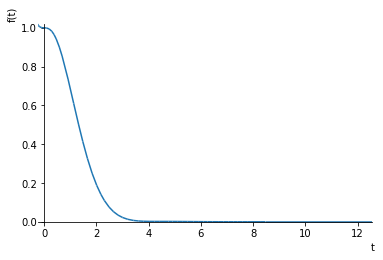
\includegraphics{img/2ldetect/denorm.png}
\caption{png}
\end{figure}

\begin{lstlisting}
<sympy.plotting.plot.Plot at 0x7fd2b91b6a90>
\end{lstlisting}

\begin{lstlisting}[language=Python]
lossy_norm_n = lambdify(t, lossy_norm(t), "numpy")
\end{lstlisting}

\begin{lstlisting}[language=Python]
lossy_norm_n(2)
\end{lstlisting}

\[0.19265133139031912\]

\begin{lstlisting}[language=Python]
X = np.linspace(1e-6, 4*np.pi, 500)  # avoid singularity in t=0
\end{lstlisting}

\begin{lstlisting}[language=Python]
Y = lossy_norm_n(X)
\end{lstlisting}

\begin{lstlisting}[language=Python]
plt.plot(X, -np.gradient(Y, X))
\end{lstlisting}

\begin{lstlisting}
[<matplotlib.lines.Line2D at 0x7fd2b6f66390>]
\end{lstlisting}

\begin{figure}
\centering
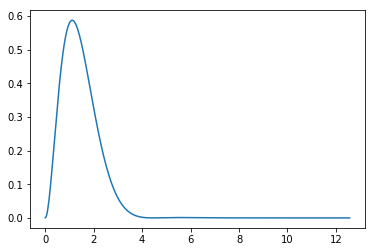
\includegraphics{img/2ldetect/prob.png}
\caption{png}
\end{figure}

\hypertarget{p-w-expectation-value-technique}{%
\subsection{P-W ``expectation value''
technique}\label{p-w-expectation-value-technique}}

\begin{lstlisting}[language=Python]
def U(_t):
    return exp(-I*H*_t)
\end{lstlisting}

\begin{lstlisting}[language=Python]
def psi_unitary(_t):
    psi = U(_t) * Matrix([1,0])
    return psi
\end{lstlisting}

\begin{lstlisting}[language=Python]
psi_unitary(t)
\end{lstlisting}

\[\left[\begin{matrix}\frac{e^{i t}}{2} + \frac{1}{2} e^{- i t}\\- \frac{e^{i t}}{2} + \frac{1}{2} e^{- i t}\end{matrix}\right]\]

\begin{lstlisting}[language=Python]
psi_unitary(t).dot( D(2*sqrt(2)) * psi_unitary(t) )
\end{lstlisting}

\[\sqrt{2} \left(- \frac{e^{i t}}{2} + \frac{1}{2} e^{- i t}\right)^{2}\]

\begin{lstlisting}[language=Python]
D(2*sqrt(2))
\end{lstlisting}

\[\left[\begin{matrix}0 & 0\\0 & \sqrt{2}\end{matrix}\right]\]

\begin{lstlisting}[language=Python]
plot(sqrt(2)* sin(t)**2 * exp(sin(t)*cos(t)/2) * exp(-t/2), (t, 0, 4*pi))
\end{lstlisting}

\begin{figure}
\centering
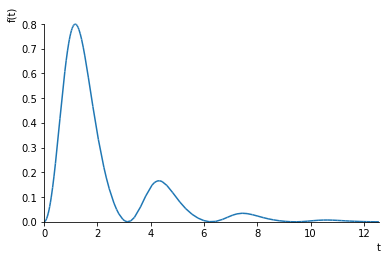
\includegraphics{img/2ldetect/prob_pw_expvD.png}
\caption{png}
\end{figure}

\begin{lstlisting}
<sympy.plotting.plot.Plot at 0x7fd2b6ef2550>
\end{lstlisting}

